Together with the company \textbf{VisCheck GmbH}, an operating unit is developed
for entering parameters on the operating terminal and reading relevant values on the operating
terminal of the bending machine. The unit consists of a franka emika robot, a camera for reading terminal values
and a computer for controlling the robot. A touch screen pointer is attached to the gripper of the robot
for operating the touch screen of terminal.

\begin{figure}[h]
    \centering
    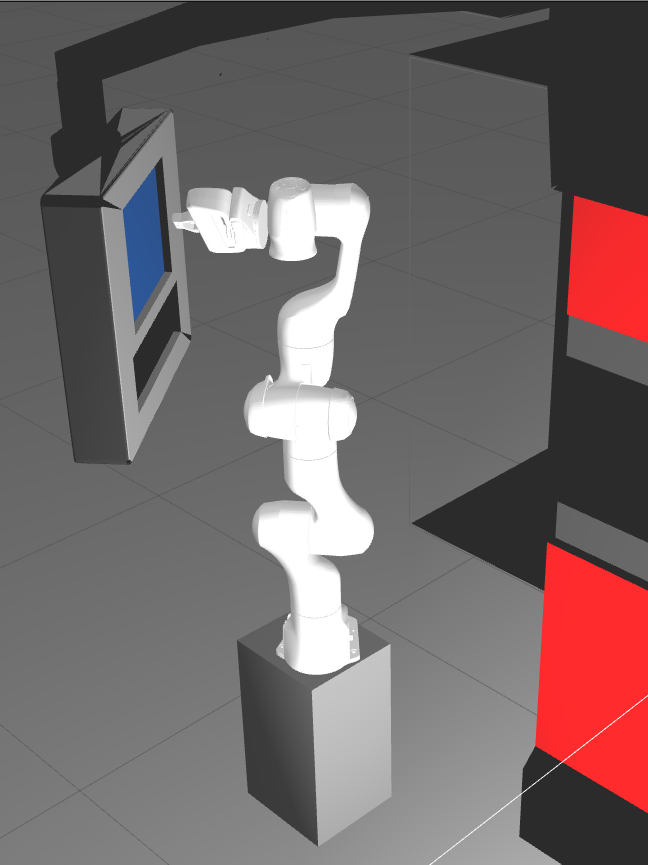
\includegraphics[width=0.3\textwidth]{figures/panda-robot-simulation.png}
    \caption{Franka emika panda robot as terminal operating robot in simulation}
    \label{fig:terminal-robot}
\end{figure}

As it is programmed by another company, it is not simulated in the software and not coordinated for any trajectory planning. Sufficient floor space
is left near the terminal of bending machine in the robotic workcell for the installation of this robot.
The trajectories of handling robot are not planned anywhere near this robot. To setup this, safety zone is created
during the programming of the handling robot.
